\begin{ZhChapter}

\chapter{緒論}

\section{研究背景}

科技的快速進步,讓人們的生活更加便利,物聯網(IoT)的應用已經與日常生活密不可分,包含了醫療及工業的應用,無所不在,\cite{mordor2024iot}根據日商環球訊息有限公司(GII)調查,物聯網(IoT)市場規模預計從2024年到2029年,將從1.17兆美元增加至2.37兆美元,年均複合成長率(CAGR)為15.12\%,如圖\ref{IoT市場規模評估}所示。

\begin{figure}[H]
    \centering
    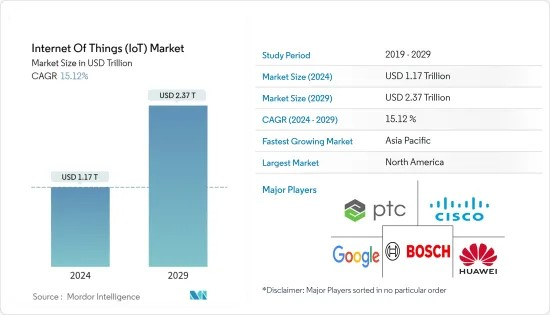
\includegraphics[width = 1\textwidth]{image/market_research.jpg}
    \caption{IoT市場規模評估\cite{mordor2024iot}}
    \label{fig: IoT市場規模評估}
\end{figure}

2010年6月藍牙技術聯盟(Bluetooth Special Interest Group)提出了低功耗藍牙(Bluetooth Low Energy, BLE),BLE省電及低成本的特性,使得藍牙技術在物聯網(IoT)的應用種佔據了不可或缺的角色,例如:目前市面上的無線設備包括藍牙耳機、藍牙鍵盤及藍牙滑鼠。
物聯網(IoT)的應用中,大量使用無線感測網路(Wireless Sensor Networks, WSN),會在環境之中分布許多的節點,而節點不只有當作感知器測量環境的數據,常常還要當作中繼節點,轉傳發送端與目的端的封包,最終將所有量測的數據匯集到終端節點,以監控所有的節點數據,將數據儲存後,進行分析後並做出適當的處理,也可以透過分析數據預測環境的變化,並提前做出適當的處理。

藍牙網狀網路(Bluetooth Mesh)架構的實現,讓BLE更具有可靠性(Reliability)及擴展性(Scalability),可以允許多個BLE相互連接並形成網狀結構,讓封包可以在多個裝置或節點之間進行傳輸,讓傳輸距離不會受到單一裝置的傳輸範圍限制,解決了節點之間裝置連接數量的限制以及傳輸距離不足的問題,在物聯網(IoT)的應用,例如:智慧建築、智慧工業、智慧城市、智慧家庭..等等,BLE都已經扮演重要也不可或缺的角色。
	
在物聯網(IoT)與藍牙網狀網路(Bluetooth Mesh)中,對整個系統架構做出適當的評估,在不影響裝置效能的情況下,設計多個藍牙裝置之間的分流機制,因為在整個系統中,流量可能會有所起伏,為了讓每個裝置可以有一樣的傳輸品質,且系統可以發揮最好的吞吐量。
	

\section{研究動機與目的}

根據文獻\cite{112TIT00392032}中針對Multi-Hop的提出DOT及DOST排程設計,研究發現在原生FruityMesh上封包傳輸是採用廣播的方式,向相鄰的所有節點發送封包,這種設計雖然簡單,卻容易導致大量冗餘封包的產生,這會導致節點之間傳輸不必要的封包,最終導致整個BLE Mesh出現廣播風暴。

\cite{112TIT00392032}作者針對FruityMesh傳輸時產生的廣播風暴,提出了DOT(Destination Oriented Transmission)排程的機制,將BLE Mesh導入樹狀結構,對整個系統進行分層管理,讓封包傳輸只會向正確的路徑上傳輸,避免了廣播風暴的產生,但是作者在研究過程中,也發現BLE Multi-Hop網狀網路節點會擁有Master以及Slave兩種角色,而在同一個時間下,節點同時會是Master和Slave的狀態,而這種狀態上的衝突會導致的封包傳輸產生遺失現象。

\cite{112TIT00392032}作者為了解決角色衝突的問題,在DOT的架構下增加啟用以及禁用的機制,提出DOST(Destination Oriented Switch Transmission)的排程設計,利用TDMA讓裝置在同一個時間只會扮演Master或Slave,解決在同一個時間點節點可能會因為扮演Master及Slave角色衝突而導致的封包傳輸遺失的問題;在研究\cite{112TIT00392032}中作者在FruityMesh中導入DOST設計,改善了大部分的封包傳輸延遲以及封包重傳率,但仍存在些許效能瓶頸,因為在FruityMesh中,所有節點的封包傳輸都是透過廣播的方式進行,這會導致在多個節點同時傳輸封包時,可能會產生封包碰撞的問題,導致封包傳輸延遲增加。


此外,文獻指出,若要在 DOST 架構下進一步提升效能,需確保拓樸建立時,Sink 節點為整體網路的根節點。然而原研究並未針對拓樸控制機制提出具體解法。若未能確保 Sink 位於樹根,當其斷線並重新加入網路時,可能無法恢復為原先的根節點角色,進而影響整體傳輸路徑的穩定性與效能。

在\cite{112TIT00392032}\cite{110TIT00392037}中,針對了single hop mesh 及 multi hop mesh的網路拓樸進行探討,當使用合適的封包連接參數可以有效降低封包傳輸延遲及重傳率,但是數據實際上傳輸時,每個封包大小並不固定,\cite{109TIT00392031}中,探討了不同封包大小可以算出最適合的連接參數,在傳輸過程動態調整連接的CE(Connection Event)及CI(Connection Interval),達到更好的吞吐量。

本計畫將研究中在DOT的排程設計下,仍然會有些許因為封包遺失,而產生的封包重傳的問題,以及在藍牙網狀網路(Bluetooth Mesh)架構,執行TDMA的排程機制,結合調整連線數據,透過修改Connection Interval數值,確保傳輸品質及確保系統可以產生最大吞吐量,並修改FruityMesh拓樸方法,讓BLE Mesh建立的過程確保Sink點在整個樹狀結構的根節點,也確保Sink點如果斷線後重新連線後依然是整個BLE Mesh樹狀結構的根節點。

\section{論文架構}



\end{ZhChapter}